\documentclass{article}
\usepackage{graphicx}
\usepackage{amsmath}
\usepackage{tikz}
\usepackage{qtree}
\usetikzlibrary{calc,shapes.multipart,chains,arrows}
\graphicspath{ {./images/} }
\title{Scheduling Solution }
\begin{document}
\maketitle
\newpage
\section*{A.3}
\subsection*{A.3.1}
To transform problem A.3 into a graph colouring problem , the problem is represented as a graph where:
\newline
Nodes = individual classes $(C_1,..., C_7)$
\newline
Edges = classes with at least one shared student (eg. "Amy" in $C_1$ and $C_5$)
\newline
Colour = A timeslot
\newline
A representation of the graph as an adjacency matrix is:
\newline
\begin{center}
$\begin{pmatrix}
   0&1&1&0&1&1&0\\
   1&0&1&0&0&1&1\\
   1&1&0&0&0&1&0\\
   0&0&0&0&1&1&0\\
   1&0&0&1&0&1&1\\
   1&1&1&1&1&0&0\\
   0&1&0&0&1&0&0\\
\end{pmatrix}$
\end{center}
An example graph would be:
\newline
\begin{center}
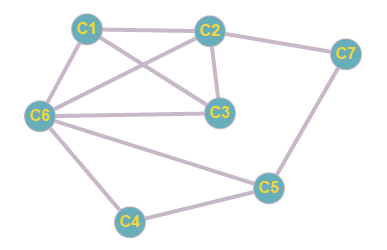
\includegraphics{a31NC}
\newline
\end{center}
The solution to the problem is the answer to the question, can the graph be coloured in at most 4 colours?
\newline
This will solve the problem because if the graph can be coloured so that no neighbouring nodes have the same timeslot then the student can physially attend every class, and by doing it in at most 4 colours means there are sufficient time slots.
\newline
An example colouring of the above graph would be:
\begin{center}
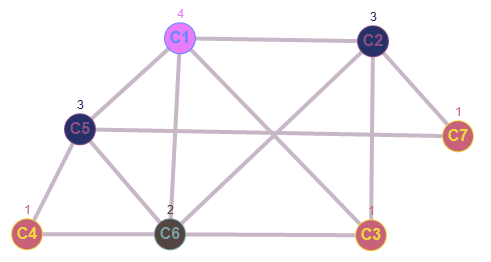
\includegraphics{a31C}
\end{center}
\subsection*{A.3.2}
As there are currently no visited nodes, the algorithm will first visit node $C_1$.
\begin{center}
Visited - $C_1$
\newline
Adjacent - $C_2,C_3,C_5,C_6$
\newline
\end{center}
Visit $C_2$
\begin{center}
Visited - $C_1,C_2$
\newline
Adjacent - $C_3,C_5,C_6,C_7$
\newline
\end{center}
Visit $C_3$
\begin{center}
Visited - $C_1,C_2,C_3$
\newline
Adjacent - $C_5,C_6,C_7$
\newline
\end{center}
Visit $C_5$
\begin{center}
Visited - $C_1,C_2,C_3,C_5$
\newline
Adjacent - $C_4,C_6,C_7$
\newline
\end{center}
Visit $C_4$
\begin{center}
Visited - $C_1,C_2,C_3,C_5,C_4$
\newline
Adjacent - $C_6,C_7$
\end{center}
Visit $C_6$
\begin{center}
Visited - $C_1,C_2,C_3,C_5,C_4,C_6$
\newline
Adjacent - $C_7$
\end{center}
Visit $C_7$
\begin{center}
Visited - $C_1,C_2,C_3,C_5,C_4,C_6,C_7$
\newline
\end{center}
Order in which the algorithm visits the vertices to find a proper colouring is:
\newline
\begin{center}
$C_1,C_2,C_3,C_5,C_4,C_6,C_7$
\end{center}
\subsection*{A.3.3}
The colours the algorithm assigns to each vertex are below:
\begin{center}
\begin{tabular}{ |c|c| }
\hline
Vertex & Colour \\
\hline
$C_1$  & 1      \\
$C_2$  & 2      \\
$C_3$  & 3      \\
$C_4$  & 1      \\
$C_5$  & 2      \\
$C_6$  & 4      \\
$C_7$  & 1       \\
\hline
\end{tabular}
\end{center}
\subsection*{A.3.4}
The chromatic number of G, $\chi$G, is 4 because it the minimum number of colours needed to properly colour G is 4.
\newline
This is because of the subgraph C1,C2,C3,C6 which looks like:
\newline
\begin{center}
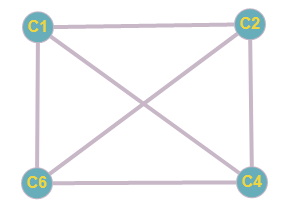
\includegraphics{a34}
\end{center}
Because this subgraph is a complete graph with 4 vertices this graph will require a minimum of 4 colours.
\begin{center}
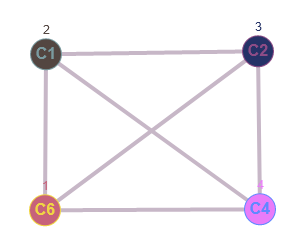
\includegraphics{a34c}
\end{center}

\end{document}